\section{OpenGL}

\subsection{Historie OpenGL}

Do devadesátých let minulého století panovalo všeobecné nadšení
z výpočetního výkonu počítačů dovolujícího kreslit 3D grafiku. Byla řada výrobců hardware. Bohužel byla i velká řada výrobců vytvářejících vlastní grafické knihovny a ovladače. Žádný tak neuměl zacházet s jakýmkoli hardwarem a měl tedy jen malou omezenou množinu aplikací.
Vznikla tak nutnost unifikace.


V další dekádě byla špičkou v grafice společnost \emph{SGI}. Vyvinula svůj standard \emph{IrisGL}. Jeho nevýhodou bylo začlenění funkcí pro \emph{X11} a použití patentovaných algoritmů. Proto začali ostatní výrobci pracovat na rozhraní od \emph{IrisGL} odvozeném a~nazvali jej \emph{OpenGL}.


V roce 1992 bylo pro účely správy \emph{OpenGL} vytvořeno konsorcium
\emph{OpenGL} ARB.	V roce 2006 byla \emph{OpenGL} předána konsorciu \emph{Kronos Group}.

\subsection{Vykreslovací řetězec}

\emph{OpenGL} popíšu jen lehkým úvodem. Začnu s popisem vykreslovacího řetězce, jak jej uvedli Procházka, Koubek a a Andrýsková v \cite{mendelu}. V současných verzích \emph{OpenGL} je ještě složitější, takto odpovídá verzi \emph{OpenGL}
2.0.

\begin{figure}[hbt]
  \begin{center}
    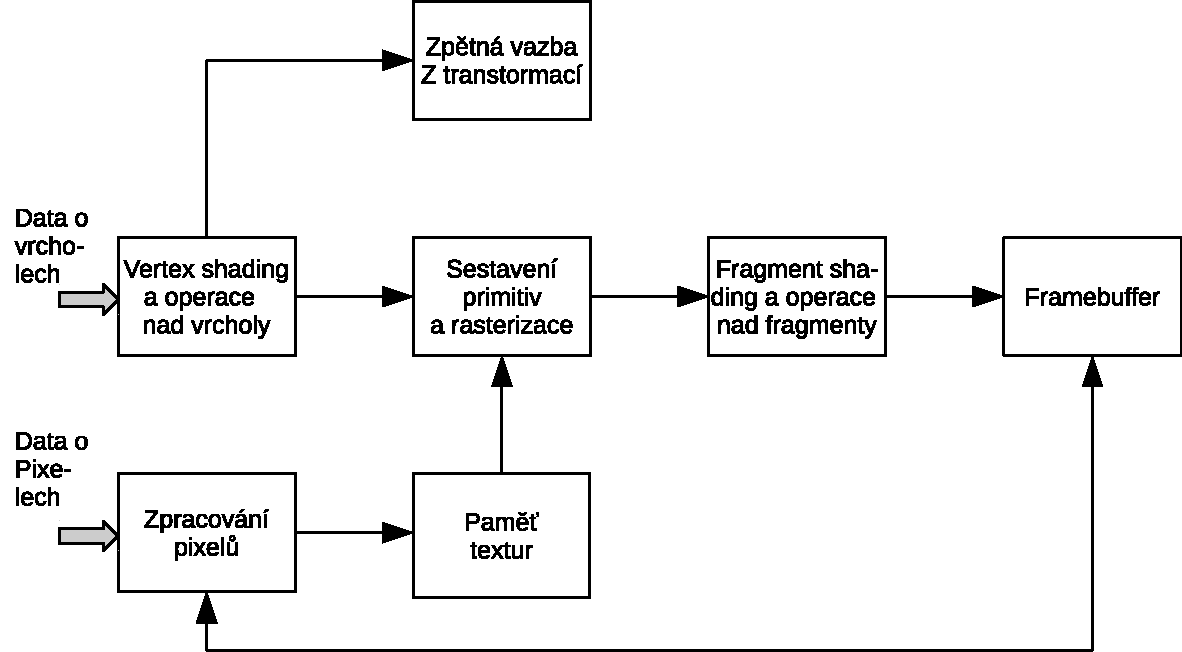
\includegraphics[scale=.6]{obr/opengl}
  \end{center}
  \caption{\emph{OpenGL} vykreslovací řetězec}
  \label{obr:openclglassdiagram}
\end{figure}

\subsubsection{Framebuffer}

Framebuffer je paměť jejíž obraz je bude zobrazen. Framebuffery jsou většinou dva nebo více, jeden se synchronně posílá na zobrazovací zařízení, ve druhém
je tvořen následující snímek.

\subsubsection{Zpracování pixelů}

Grafický subsystém, jakožto rasterové zařízení umožňuje práci s rasterovými daty. V postatě je schopen je jen zapsat/vyčíst framebufferu a zapsat do paměti textur.

\subsubsection{Zpracování vrcholů}

Vrchol (vertex) není jen bod v prostoru. V \emph{OpenGL} má vertex kromě své pozice řadu dalších uživatelských vlastností, které lze z programu nastavit a také je při zpracování vrcholu využít. Dříve byla tato jednotka fixní, grafický čip prováděl vždy stejnou operaci nad vrcholy. Nyní, od \emph{OpenGL} 2.0, je vykreslovací řetězec programovatelný a tato jednotka může vykonávat s vrcholem jakoukoli operaci pomocí programu v jazyce \emph{GLSL}. Lze tak realizovat základní operace s vrcholem, jako otočení, změna měřítka, posunutí, ale i třeba efekty jako jsou vlny na hladině, efekt lomení paprsku na hladině a podobně.

\subsubsection{Sestavení primitiv a rasterizace}

Když předchozí jednotka stanovila již definitivní souřadnice ploch, je třeba z každé jednotlivé plochy
získat množinu bodů, které odpovídají pixelům na zobrazovacím zařízení, fragmentům.

\subsubsection{Fragment shading a operace nad fragmenty}

Stejně jako vertex není jen bod v prostoru, tak i fragment obsahuje více informací než jen polohu a barvu. Tato jednotka je od \emph{OpenGL} 2.0 programovatelná v jazyce \emph{GLSL} a umožňuje nanášet textury, vybarvovat pixel podle jeho polohy (barevný přechod), některé efekty se světlem, míchání barev a podobně.
